%! TEX Root = _main.tex
\section{はじめに}
調推定（key estimation）は，楽譜や演奏音の全体または局所区間から，長調・短調と主音の組であるkey labelを得る課題である．その出力は，楽曲の調を外部から記述する．

これに対し，本研究が対象とするのは，歌唱者が現在どの音をドと捉え，周囲の音をどの枠組みで解釈しているかという内的な状態，すなわち主観的調性感（Subjective Tonality）である．目的はkey labelの付与ではなく，任意の音高から始まる歌唱に対して，主観主音を基準とする枠組みを継続的に保持・更新することにある．

そこで，主観的調性感の内部表現としてRelative Tonal Frame（RTF）を導入し，RTFに基づく一人合唱とのインタラクションを通して動的な調性感を体験するシステムを提案する．

\section{関連研究}
key estimationの背景には，文脈に応じて各音の適合度が異なるという調性階層の知見がある．Krumhanslらはtone profileによる調相互の認知的関係と，和音列に伴う調的組織の知覚変化を報告した\cite{Krumhansl1982}．本研究は知覚一般の説明ではなく，歌唱インタラクションに用いる内部状態の表現を目的とする．

ChewのSpiral Arrayはpitch，chord，keyの関係を幾何学的に扱う計算モデルであり\cite{Chew2014}，LerdahlのTonal Pitch Spaceはpitch，chord，region間の階層的距離を理論化する\cite{TPS}．これらが調的要素間の関係を記述するのに対し，RTFはSubjective Tonicを原点として，個々の歌唱者の主観的調性感を保持・更新する相対的な内部表現である．

HarmoSoloは一人アカペラをリアルタイムにハーモナイズする\cite{tokunaga2026}．本研究はこの文脈を共有しつつ，生成声部の基準となる主観的調性感をRTFとして明示し，その変化の体験に焦点を置く．

\section{主観的調性感とRelative Tonal Frame}
本研究では，歌唱者が歌唱中に形成・維持・更新すると想定する調性の認知状態を\textbf{主観的調性感（Subjective Tonality）}と呼ぶ．

これは直接観測できないため，\textbf{Relative Tonal Frame}（RTF）を内部表現として用いる．RTFはSubjective Tonic（主観主音）を原点とし，各音を相対的位置として表す．Subjective Tonalityが認知的概念であるのに対し，RTFはシステムが操作する状態表現であり，開始音高が異なる同一旋律を同じ相対関係として扱える．

本システムは，歌唱を説明する内部状態としてRTFを推定・更新する．Tonality Operatorは，音高系列の特徴量から，RTFを維持・調整・再形成する根拠を評価する．

\begin{figure*}[t]
    \centering
    \begin{minipage}{0.515\textwidth}
        \centering
        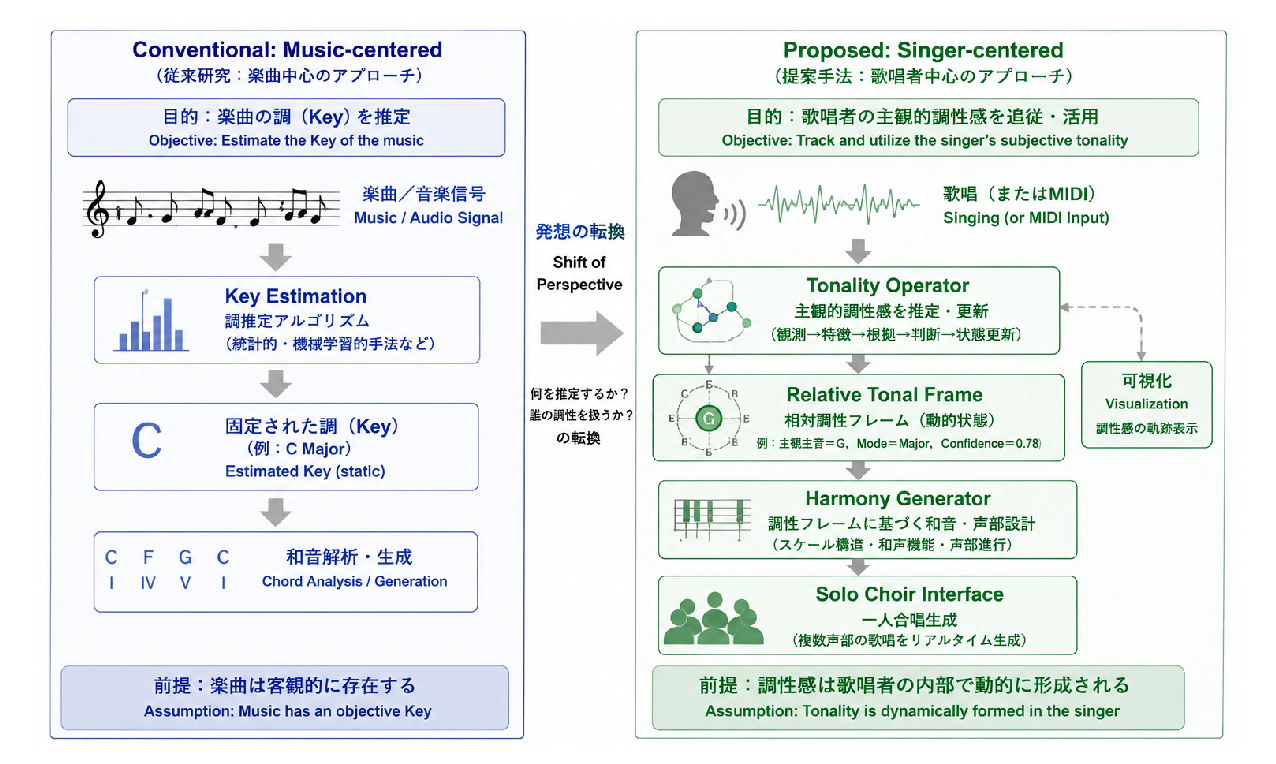
\includegraphics[width=\linewidth]{fig/fig1_concept.pdf}
        \caption{主観的調性感の概念図}\label{fig:concept}
    \end{minipage}
    \hfill
    \begin{minipage}{0.48\textwidth}
        \centering
        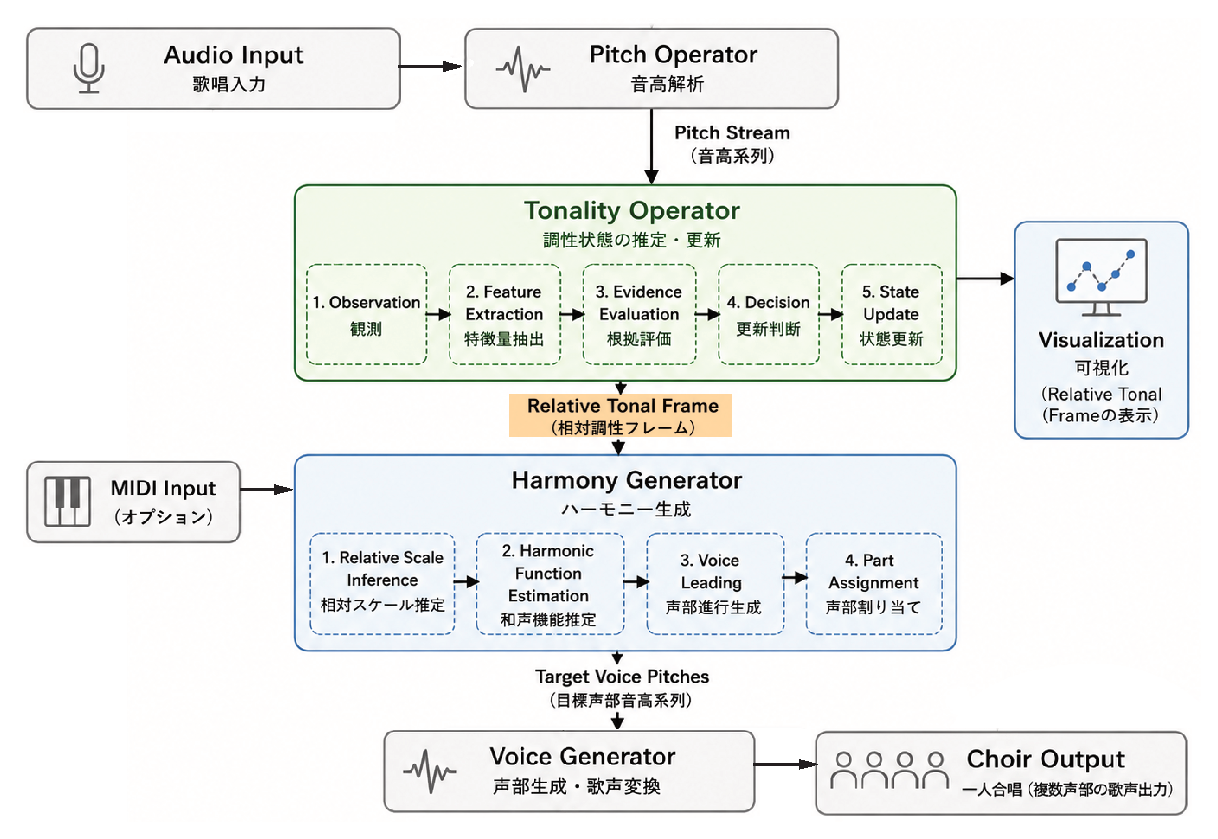
\includegraphics[width=\linewidth]{fig/fig2_system.pdf}
        \caption{システム構成}\label{fig:system}
    \end{minipage}
\end{figure*}


\section{システム構成}

\figref{fig:system}にシステム全体の構成を示す．
本システムは，
歌唱またはMIDI入力から音高系列を取得するPitch Operator，
主観的調性感の内部表現であるRTFを推定・更新するTonality Operator，
推定されたRTFに基づいて各声部の目標音高を決定するHarmony Generator，
および複数声部の歌唱を生成するVoice Generatorから構成される．この順に観測，RTF更新，声部決定，音声生成を行う．RTFは主観的調性感を表す調性状態として後段から参照される．


\subsection{Tonality Operator}

Tonality Operatorは，音高系列から現在の歌唱を説明するRTFを推定し，内部状態として保持する．

音高観測，特徴量抽出，Evidence算出，状態更新判断，状態更新の責務を分離し，RTFを変更する判断と実際の更新を区別する．

\subsection{Harmony Generator}

Harmony GeneratorはRTFを参照し，スケール構造と基本的な和声進行に基づいて各声部の目標音高を決定する．

Voice Generatorは入力歌唱を各目標音高へ変換し，一人の歌唱から複数声部を生成する．これにより，主観的調性感の内部表現であるRTFをハーモニーへ反映する．

\section{デモ展示}

参加者は任意の音高から歌唱し，固定的なkey labelではなく，Subjective Tonicからの相対関係を表すRTFに基づく一人合唱を体験する．

異なる開始音高から同一旋律を歌唱するとともに，主観的調性感の内部表現であるRTFを可視化し，生成ハーモニーとの対応を提示する．

これにより，固定的な調名の正誤ではなく，歌唱に伴って相対的な枠組みが更新される観点から，主観的調性感と生成音の関係を体験する．



\section{おわりに}

本稿では，key labelを求めるkey estimationとは異なり，主観的調性感の内部表現としてRTFを継続的に扱う一人合唱インタフェースを紹介した．RTFと生成合唱の対応を通して，動的な調性感に基づく歌唱インタラクションの可能性を議論する．
